\documentclass[12pt]{article}
\usepackage[letterpaper,left=2.25cm,top=3.0cm,right=2.25cm,bottom=2.0cm, headsep=1.5cm]{geometry}
\usepackage{fancyhdr}
\usepackage[utf8]{inputenc}
\usepackage[T1]{fontenc}
\usepackage[spanish,mexico]{babel}
%\usepackage[letterpaper,margin=2.5cm]{geometry}
\usepackage{setspace}
\usepackage{titlesec}
\usepackage{tocloft}
\usepackage{graphicx}
\usepackage{longtable}
\usepackage{csquotes}
\setlength{\headheight}{47pt}
\usepackage[linguistics]{forest}
\usepackage{amssymb, amsmath, amsbsy} % simbolitos


\setcounter{secnumdepth}{4} % Permite numerar hasta el cuarto nivel (paragraph)
\setcounter{tocdepth}{4}    % Permite que el cuarto nivel aparezca en el índice

\usepackage{xcolor}
\usepackage{multirow}
\usepackage{listings}
\usepackage{caption}
\usepackage{subcaption}
%\usepackage{parskip}
\usepackage[skip=12pt plus1pt]{parskip}
\usepackage{pdfpages} % Incluir PDF en documento en LATEX
\usepackage{verbatim} % comentarios
\usepackage{algpseudocode}
\usepackage{algorithm}
\usepackage{pdflscape}
\usepackage{afterpage}
\usepackage{array,booktabs,ragged2e}
\usepackage{rotating}
%\usepackage{hyperref}
\usepackage{wallpaper}
% \newcolumntype{C}[1]{>{\centering\arraybackslash}p{#1}} % Centrar }
\newcolumntype{L}[1]{>{\raggedright\let\newline\\\arraybackslash\hspace{0pt}}m{#1}}
\newcolumntype{C}[1]{>{\centering\let\newline\\\arraybackslash\hspace{0pt}}m{#1}}
\newcolumntype{R}[1]{>{\raggedleft\let\newline\\\arraybackslash\hspace{0pt}}m{#1}}




% Para utilizar el formato de citas IEEE y comentar los dos parrafos siguientes. Ademas de utilizar el comando \cite en vez de \cite
\usepackage[backend=biber,sorting=none]{biblatex}
% Para utilizar el formato APA, sugiero comentar la linea anterior y descomentar las dos proximas lineas. Ademas de utilizar el comando \cite en vez de \cite
%\usepackage[backend=biber,style=apa]{biblatex}
%\DeclareLanguageMapping{english}{american-apa}

\makeatletter
\DefineBibliographyExtras{spanish}{%
  \setcounter{smartand}{1}%
  \let\lbx@finalnamedelim=\lbx@es@smartand
  \let\lbx@finallistdelim=\lbx@es@smartand
}
\renewbibmacro*{name:delim:apa:family-given}[1]{%
  \ifnumgreater{\value{listcount}}{\value{liststart}}
    {\ifboolexpr{
       test {\ifnumless{\value{listcount}}{\value{liststop}}}
       or
       test \ifmorenames
     }
       {\printdelim{multinamedelim}}
       {\lbx@finalnamedelim{#1}}}
    {}}
\makeatother
% Estas lineas permiten romper los hipervinculos muy largos en las referencias!!!!
\setcounter{biburllcpenalty}{7000}
\setcounter{biburlucpenalty}{8000}
\addbibresource{Referencias.bib} % ARCHIVO DE BIBLIOGRAFÍA


\usepackage[bookmarks=true,breaklinks=true,bookmarksopen=false,colorlinks=true,linkcolor=blue]{hyperref}
\usepackage[hyphenbreaks]{breakurl}
\usepackage{pdfpages} % Incluir PDF en documento en LATEX
\setstretch{1.3}

\usepackage{soul}


% CONSTANTES NECESARIAS PARA EL DOCUMENTO ---> MODIFIQUEN A SU CRITERIO
\newcommand{\NombreAlumno}{Valeria Mayrín Bermúdez Raga}
\soulregister{\NombreAlumno}{1}
% NUNCA PONGAN EL TITULO EN MAYUSCULAS!!
\newcommand{\NombreProyecto}{Sistema Web de Gestión y Actualización de Datos del Personal del PJETAM} 
% Noten los \\ para insertar un ENTER del texto en el encabezado. NUNCA PONGAN EL TITULO EN MAYUSCULAS!!
\newcommand{\NombreProyectoheader}{Sistema Web de Gestión y Actualización de Datos del Personal del PJETAM}
\newcommand{\NombreTSU}{Desarrollo de Software Multiplataforma}
\newcommand{\UnidadEconomica}{Supremo Tribunal de Justicia del Estado de Tamaulipas}
\newcommand{\nasesorempresaria}   {Ing. Luis Roberto Flores de la Fuente}
\newcommand{\nasesorinstitucional}{Dr. Said Polanco Martagón}
\newcommand{\Matricula}           {2430215}  %SU MATRICULA
\newcommand{\ncuatrimestre}{Mayo-Agosto 2026}
% ESTA ES LA FECHA EN LA QUE EL ASESOR INSTITUCIONA EVALUA EL INFORME
\newcommand{\fechaAutorizacionInforme}               {31 de Julio de 2026} 
% ESTA ES LA FECHA EN LA QUE EL ASESOR INSTITUCIONA PROGRAMA LA EXPOSCION 
\newcommand{\DiaEvaluacionPesentacion}{12}
\newcommand{\MesEvaluacionPesentacion}{Agosto}
\newcommand{\AnhoEvaluacionPesentacion}{2026}
\newcommand{\fechaPortada}               {\MesEvaluacionPesentacion~de~\AnhoEvaluacionPesentacion}
\newcommand{\HoraEvaluacionPesentacion}{10:00 hrs}

\newcommand{\modalidadEvaluacionPesentacion}{Presencial} % Otras opciones: Virtual
\newcommand{\tipoAulaOficinaEnlacePesentacion}{la Oficina} % Otras opciones: la oficia/el aula/enlace
\newcommand{\AulaEvaluacionOEnlaceMeetPesentacion}{I-XXX69} %otras opciones: si es un elance de meet, rodearlo \url{}

%\newcommand{\modalidadEvaluacionPesentacion}{Virtual} % Otras opciones: Virtual
%\newcommand{\tipoAulaOficinaEnlacePesentacion}{el enlace} % Otras opciones: la oficia/el aula/el enlace
%\newcommand{\AulaEvaluacionOEnlaceMeetPesentacion}{\url{http://www.upvictoria.edu.mx}} %otras opciones: si es un elance de meet, rodearlo \url{}

\newcommand{\ncarrera}            {Ingeniería en Tecnologías de la Información e Innovación Digital}


\fancyhead{} % Clear all header fields
\fancyhead[C]{%
    \begin{tabular}{@{} m{0.2\textwidth} m{0.5\textwidth} m{0.2\textwidth} @{}}
        % Left image
        \includegraphics[height=1.20cm]{UTYP.png}
        &
        % Center text (multiline, centered)
        \centering
        \scriptsize{\NombreProyectoheader}
        %\textbf{University Name} \\ 
        %Department of Something \\ 
        %Course Title
        &
        % Right image
        %\raggedleft
        \includegraphics[height=1.5cm]{LogoUPV_2023.png}
    \end{tabular}
}


%\usepackage{imakeidx}
%\makeindex[title=New Index Title]

%\renewcommand{\contentsname}{Whatever}
%

%\usepackage[english]{babel}

\addto\captionsspanish{% Replace "english" with the language you use
  \renewcommand{\contentsname}%
    {Contenido temático}%
}


\renewcommand\spanishtablename{Tabla}

\begin{document}

% PAGINA 1 - PORTADA
\setcounter{page}{0}
\pagenumbering{roman}
\thispagestyle{empty}




\begin{titlepage}


\vspace*{-2cm}
\begin{center}
\begin{tabular}{cp{6cm}c}
\includegraphics[height=2.25cm]{UTYP.png} & 
& \includegraphics[height=2.25cm]{LogoUPV_2023.png}   \\
\end{tabular} \\[0.5cm]



{\Large \textbf{UNIVERSIDAD POLITÉCNICA DE VICTORIA}}\\[1.0cm]

{\Large \textbf{REPORTE DE ACTIVIDADES DEL PROYECTO}}\\[0.75cm]

{\Large \MakeUppercase{\NombreProyecto}}\\[1.0cm]

QUE PRESENTA

\textbf{\MakeUppercase{\NombreAlumno}}\\[1.0cm]

EN CUMPLIMIENTO DE LA ESTADÍA TSU EN\\
\textbf{\MakeUppercase{\NombreTSU}}\\[0.75cm]

ASESOR INSTITUCIONAL\\
\textbf{\MakeUppercase{\nasesorinstitucional}}\\[0.5cm]

UNIDAD ECONÓMICA RECEPTORA:\\
\textbf{\MakeUppercase{\UnidadEconomica}}\\[0.5cm]

ASESOR DE LA UNIDAD ECONÓMICA\\
\textbf{\MakeUppercase{\nasesorempresaria}}\\[0.5cm]


\end{center}
\begin{flushright}
Ciudad Victoria, Tamaulipas, \fechaPortada.
\end{flushright}

\end{titlepage}


\newpage
% PAGINA 1 - PORTADA
\setcounter{page}{0}
\pagenumbering{roman}
\pagestyle{empty}
\ULCornerWallPaper{1}{Membrete2023.pdf}
\vspace*{2cm}



\begin{center}
{\Large \textbf{Formato de autorización para exposición de Estadía de}}\\[0.125cm]
{\Large \textbf{Técnico Superior Universitario}}\\[0.25cm]
\end{center}

\noindent
Fecha y lugar en que se emite: \textbf{Ciudad Victoria, Tamaulipas, a \fechaAutorizacionInforme } \\[0.125cm]
Nombre completo del estudiante: \textbf{\NombreAlumno} \\[0.125cm]
Matrícula: \textbf{\Matricula}  \\[0.125cm]
Programa Académico: \textbf{\ncarrera}  \\[0.25cm]

\noindent
Por medio del presente, se le informa que tras realizar su Estadía en la empresa \textbf{\UnidadEconomica} llevando a cabo el proyecto: \textbf{\NombreProyecto}, durante el periodo comprendido \textbf{\ncuatrimestre} logrando una ponderación de \_\_\_\_  (60\% posibles) para el criterio de reporte; por lo tanto, se otorga la oportunidad de exponer el trabajo realizado por medio de un informe ejecutivo programado para el día \textbf{\DiaEvaluacionPesentacion} del mes de \textbf{\MesEvaluacionPesentacion} del año en curso en un horario de \textbf{\HoraEvaluacionPesentacion} en modalidad \textbf{\modalidadEvaluacionPesentacion} en \textbf{\tipoAulaOficinaEnlacePesentacion} \textbf{\AulaEvaluacionOEnlaceMeetPesentacion}.

\vspace{0.25cm}

\noindent
Sin otro particular, se le recomienda estar disponible para iniciar su exposición 10 minutos antes de la indicación oficial.

\vspace{0.5cm}

\begin{center}
\begin{tabular}{p{10cm}}
\multicolumn{1}{c}{Atentamente}   \\
 \\
 \\ \hline
\multicolumn{1}{c}{\nasesorinstitucional}   \\
\multicolumn{1}{c}{Asesor institucional}   \\
\end{tabular}
\end{center}

\clearpage
\ULCornerWallPaper{1}{Membrete2023.pdf}

\vspace*{3cm}

\begin{center}
{\large \textbf{Control sumativo de Estadía para Técnico Superior Universitario}}
\end{center}

\vspace{0.5cm}

\begin{center}
\begin{tabular}{|p{6cm}|p{4cm}|p{4cm}|}
\hline
\textbf{Criterio} & \textbf{Valor / Ponderación} & \textbf{Calificación} \\ \hline
Reporte & 60\% & \\ \hline
Exposición & 40\% & \\ \hline
Calificación final & \multicolumn{2}{c|}{ } \\ \hline
\end{tabular}
\end{center}

\vspace{0.8cm}

%\noindent
%\textbf{Nota:} para completar este documento deberá sustentar su decisión con base en las rúbricas oficiales de la institución diseñadas para cada evaluación.

\begin{center}
\begin{tabular}{|p{10cm}|}
\hline
\multicolumn{1}{|c|}{\textbf{Datos de la evaluación sumativa}}\\
\multicolumn{1}{|c|}{Fecha: \textbf{\DiaEvaluacionPesentacion}  / \textbf{\MesEvaluacionPesentacion} / \textbf{\AnhoEvaluacionPesentacion}} \\ \hline
%\multicolumn{1}{c}{Atentamente}   \\
 \\
 \\ \hline
\multicolumn{1}{c}{\nasesorinstitucional}   \\
\multicolumn{1}{c}{Asesor institucional}   \\
\end{tabular}
\end{center}





%\vspace{1cm}

%\noindent




%\vspace{1.5cm}

%\noindent
%Firma: \hrulefill

%\vspace{1cm}

%\noindent
%Nombre del Asesor institucional: \nasesorinstitucional \hrulefill


\clearpage
\ClearWallPaper
\thispagestyle{fancy}
\addcontentsline{toc}{section}{Resumen}
%\vspace*{1cm}
\section*{Resumen}

El resumen es una representación condensada del contenido del documento. Su propósito es dar al lector un relato de las características principales del reporte. Su redacción es en tercera persona, en tiempo pasado, con escritura continua y sin tablas o imágenes. La extensión sugerida es no mayor a media página. Debe cumplir con las siguientes características:

\begin{itemize}
\item Se hace mención del nombre del proyecto como parte de la Estadía, el nombre de la unidad económica y su dirección completa.
\item Se menciona el objetivo, meta, actividad o responsabilidad principal que se abordó.
\item Se describe detalladamente la metodología desarrollada; tales como herramientas, materiales, equipos, cursos, softwares y conocimientos adquiridos en la universidad utilizados para alcanzar los objetivos empleados.
\item Se describen detalladamente los resultados más importantes obtenidos.
\item Se termina presentando conclusiones del trabajo.
\end{itemize}


\clearpage
\thispagestyle{fancy}
\addcontentsline{toc}{section}{Abstract}
%\vspace*{1cm}
\section*{Abstract}
Add your abstract here...

\clearpage
%\renewcommand{\indexname}{Contenido temático}

\thispagestyle{empty}
\ClearWallPaper
\tableofcontents


%\chapter{Introducción}

\clearpage
\pagenumbering{arabic}
\setcounter{page}{1}
\pagestyle{fancy}

\section{Introducción}
\label{ch:introduccion}

Actualmente las instituciones gubernamentales suelen utilizar sistemas que pueden resultar ser algo anticuados ya que la mayoría fueron desarrollados hace años y continúan usando tecnologías de esa época; a simple vista, estos pueden parecer funcionales pero varios de estos pueden presentar problemas como problemas de mantenimiento, algunas limitaciones técnicas como incompatibilidad con sistemas operativos modernos y riesgos en la seguridad de los datos. 

Es necesario modernizar estos sistemas antiguos ya que mientras más pase el tiempo más cambian las necesidades y más cambian las tecnologías modernas, lo que dificulta la adopción de nuevas funciones que la empresa necesite para escalar o mejorar la atención al personal.

Tal es el caso del sistema para la gestión y actualización de datos del personal del Poder Judicial del Estado de Tamaulipas, el cual fue desarrollado hace más de 15 años, y su interfaz y funcionamiento lo demuestran. La seguridad y eficiencia en el manejo de los datos del personal garantiza la capacidad para poder mantener sus servicios funcionando y también la protección de los datos sensibles lo que ayuda a que también haya un clima de confianza entre los trabajadores y el manejo de sus datos, además de disminuir las equivocaciones asociadas a la manipulación de estos datos.

En este proyecto se busca implementar un sistema siguiendo las bases del que está ya en funcionamiento pero integrando un tipo de acceso centralizado y que pueda tener un mantenimiento sencillo a largo plazo con ayuda de desarrollo web moderno e integración de APIs, para así lograr una mejora en los procesos administrativos que realizan en el Poder Judicial del Estado de Tamaulipas.
\subsection{Antecedentes}
\label{sec:antecedentes}

\subsubsection{Antecedentes de la empresa}
\label{sec:antecedentes_empresa}

\paragraph{Información general del PJETAM} ~\\
\label{sec:informacion}El Poder Judicial del Estado de Tamaulipas es una institución pública encargada de impartir y administrar justicia en el estado de Tamaulipas. Su objetivo principal es resolver conflictos entre particulares y autoridades, garantizando el Estado de derecho, la protección de los derechos humanos y la paz social.\cite{PJETAM:ReglamentoTribunalElectronico2022}

Entre las principales funciones institucionales que este realiza se encuentran resolver conflictos entre los ciudadanos, entre empresas, o entre los particulares y el Estado, basándose en la legislación vigente. De igual forma, asegurar que ninguna ley, norma o acto de autoridad vulnere lo establecido en la Constitución y servir de salvaguarda ante violaciones a los derechos humanos y libertades individuales. Además de actuar como un contrapeso democrático para limitar el poder del Ejecutivo y del Legislativo, asegurando que sus actos se mantengan dentro del marco.\cite{PJETAM:ReglamentoTribunalElectronico2022}

\paragraph{Misión} ~\\
\label{sec:mision}Impartir y administrar justicia de manera eficiente y expedita, solucionando conflictos a través de los órganos jurisdiccionales y los medios alternos, contribuyendo a garantizar el estado de derecho y la paz social en Tamaulipas.\cite{PJETAM:MisionVision}

\paragraph{Visión} ~\\
\label{sec:vision}Transcender como Institución de excelencia, mediante la profesionalización e institucionalización de sus integrantes, en un ambiente de humanismo y justicia institucional, haciendo uso de la innovación tecnológica y optimización de los recursos, con responsabilidad social y pleno respeto a la ley, los derechos humanos y la igualdad de género.\cite{PJETAM:MisionVision}

\paragraph{Tribunal Electrónico para el manejo de datos del personal} ~\\
\label{sec:sistemas_informacion}El Poder Judicial del Estado de Tamaulipas mantiene una necesidad constante de modernizar y ampliar sus sistemas informáticos para agilizar trámites y garantizar la transparencia; esto se refiere a que es primordial tener infraestructura, software especializado y herramientas de ciberseguridad de alta calidad para el desarrollo de sus sistema informáticos. Para hacer frente a estas necesidades, la institución se apoya en el Tribunal Electrónico, un ecosistema digital que requiere soporte y desarrollo tecnológico continuo.\cite{PJETAM:ReglamentoTribunalElectronico2022}

Dentro del ecosistema del Tribunal Electrónico se encuentra el sistema para la gestión y actualización de datos del personal, el cual fue desarrollado aproximadamente hace 15 años utilizando tecnologías como el framework ASP.NET Web Forms y el lenguaje de programación Visual Basic, bajo una arquitectura en capas, separando  el diseño visual de la lógica del sistema. 
Aunque dicho sistema permitió durante varios años llevar a cabo procesos administrativos relacionados con la información del personal, con el paso del tiempo comenzaron a presentarse diversas limitaciones derivadas de la antigüedad de las tecnologías empleadas. 

Entre estas limitaciones destacan las dificultades de mantenimiento, la complejidad para implementar nuevas funcionalidades, problemas de compatibilidad con herramientas modernas y restricciones en aspectos relacionados con la seguridad y escalabilidad. Esta situación evidenció la necesidad de modernizar el sistema mediante una solución web basada en tecnologías actuales que permitieran mejorar la eficiencia operativa, la experiencia de usuario y la integración con otros servicios institucionales.
\subsubsection{Antecedentes teóricos}
\label{sec:antecedentes_teoricos}

\paragraph{Sistemas Heredados (Legacy Systems) en Administración Pública} ~\\
\label{sec:legacy_systems}El avance continuo de las tecnologías de la información provoca que sistemas informáticos que han sido utilizados por años se conviertan en sistemas heredados o legacy systems, los cuales, a pesar de presentar limitaciones técnicas u operativas, siguen vigentes porque estos tienen un alto valor y tienen datos que ya son vitales para la organización. En las organizaciones públicas, la eliminación o sustitución inmediata de estas plataformas es una tarea sumamente compleja debido al riesgo latente de interrumpir las actividades administrativas diarias y afectar directamente la continuidad de la entrega de servicios institucionales.

Con el paso de los años, mantener estos sistemas antiguos eleva considerablemente los costos de soporte técnico y aumenta la dificultad de mantenimiento debido a la escasez de expertos en herramientas obsoletas junto con una documentación de referencia que suele ser insuficiente. De acuerdo con Mandviwalla et al. (2026)\cite{mandviwalla2025modernizing}, los sistemas heredados centrales personalizados terminan atrapando las prácticas críticas de la organización y su información en un entorno técnico moribundo y rígido. Esto no solo incrementa la vulnerabilidad ante ciberataques o caídas operativas, sino que convierte al software en una "trampa de valor" que frena la innovación interna, bloquea la agilidad institucional y dificulta la consolidación limpia de los datos.

\paragraph{Limitaciones Técnicas de ASP.NET Web Forms} ~\\
\label{sec:limitaciones_aspnet}Un ejemplo de esta problemática de obsolescencia se presenta en las aplicaciones web desarrolladas bajo el entorno de ASP.NET Web Forms. Según Herceg (2024)\cite{herceg2024modernizing}, esta tecnología de generaciones previas basaba su arquitectura en componentes de servidor y en un estado persistente oculto denominado View State, el cual provocaba transferencias de datos pesadas y complejas (postbacks) hacia el servidor ante cualquier interacción del usuario. Este flujo no solo generaba problemas de parpadeo y lentitud en las interfaces disminuyendo la usabilidad, sino que introducía un fuerte acoplamiento con los componentes del sistema operativo Windows y el servidor de aplicaciones IIS (Internet Information Services).

Microsoft determinó omitir por completo el soporte para la tecnología Web Forms en las nuevas generaciones de .NET Core y .NET moderno, enfocándose exclusivamente en el desarrollo de plataformas más ligeras y eficientes. Herceg (2024)\cite{herceg2024modernizing} subraya que, debido a que no existe un marco equivalente directo en las versiones actuales, la migración de un sistema basado en Web Forms implica obligatoriamente una reingeniería profunda y la reescritura total de las páginas y elementos de la interfaz de usuario utilizando nuevas tecnologías de presentación.

\paragraph{Impacto de la Arquitectura Modelo-Vista-Controlador (MVC)} ~\\
\label{sec:impacto_mvc}Para evitar el código extenso, rígido y difícil de mantener en un proyecto, la ingeniería de software implementa ciertos patrones de diseño que nos ayudan al desarrollo de nuestros proyectos. Entre estas estructuras, se encuentra el patrón Modelo-Vista-Controlador (MVC) destaca por proponer una división modular de la aplicación en tres componentes: el modelo, encargado de la gestión y acceso a la base de datos; la vista, que es la presentación visual de la información al usuario; y el controlador, que procesa las solicitudes y dirige el flujo de la aplicación.

La utilización de este enfoque aporta ventajas significativas durante todo el ciclo de vida del sistema. Enríquez et al. (2023)\cite{enriquez2023impacto} demuestran mediante su investigación que el patrón MVC tiene un impacto positivo sobre la seguridad, la interoperabilidad y la usabilidad de las soluciones tecnológicas corporativas. Al separar la lógica de presentación de la lógica de negocio, el patrón MVC permite a los desarrolladores lograr una mayor escalabilidad, facilitar la reutilización de componentes de software y reducir la complejidad en la realización de pruebas funcionales frente a otro tipo de patrones.

\paragraph{Tabla Comparativa de Tecnologías} ~\\
\label{sec:tablacomparativa}Como se puede observar en la Tabla \ref{tab:tabla_tecnologias}, se contrastan las deficiencias tecnológicas de la plataforma actual frente a las ventajas de la propuesta de rediseño, fundamentando la necesidad de realizar la modernización en el presente.

\begin{table}[H]
    \centering
    \caption{Tabla Comparativa de Tecnologías y Justificación de Modernización.}
    \label{tab:tabla_tecnologias}
    \small
    \begin{longtable}{|p{2.8cm}|p{4.2cm}|p{4.2cm}|p{5.3cm}|}
        \hline
        \textbf{Criterio de comparación} & \textbf{ASP.NET Web Forms (Sistema Heredado)} & \textbf{Arquitectura MVC en .NET Moderno (Propuesta)} & \textbf{Motivo de la Modernización Actual (Justificación)} \\
        \hline
        Arquitectura de Software & Estructura basada en componentes de servidor rígidos y un estado persistente (View State). & Separación en tres capas independientes con responsabilidades distintas, que son: Modelo, Vista y Controlador. & Web Forms es una tecnología obsoleta que carece por completo de soporte o alternativas en las versiones actuales de .NET.\\ \hline
        Mantenibilidad y Código & Propensión a mezclar la lógica de negocio dentro del código visual. & Alta modularidad que promueve el aislamiento de las reglas del negocio, facilitando la reutilización y evolución del código. & Reducir la alta deuda técnica acumulada por más de 15 años, disminuir los costosos gastos de soporte y agilizar la integración de nuevas funciones operativas. \\ \hline
        Dependencia Tecnológica & Dependencia con componentes específicos de Windows y el servidor de aplicaciones IIS. & Diseñado de forma ligera para trabajar en entornos distribuidos o contenedores en la nube. & El entorno moderno exige agilidad multiplataforma y la capacidad técnica de responder velozmente a demandas globales de la institución. \\ \hline
        Seguridad & Uso de Membership Providers desactualizados cuyos antiguos algoritmos de cifrado ya no son seguros hoy en día. & Gestión avanzada de identidades e integración segura mediante APIs modernas y controles basados en roles. & Salvaguardar de manera estricta la información sensible del personal y mitigar riesgos cibernéticos. \\
        \hline
    \end{longtable}
\end{table}

\subsection{Definición del Problema}
\label{sec:problema}

Actualmente, el Poder Judicial del Estado de Tamaulipas cuenta con un sistema para la gestión y actualización de datos del personal desarrollado hace más de 15 años. Debido al tiempo transcurrido desde su implementación, dicho sistema presenta diversas limitaciones tecnológicas que afectan su funcionamiento, mantenimiento y capacidad de adaptación a las necesidades actuales de la institución.

Entre las principales problemáticas identificadas se encuentran el uso de tecnologías obsoletas como el framework ASP.NET Web Forms, dificultades para realizar mantenimiento o implementar nuevas funcionalidades, limitaciones en la seguridad de la información y una experiencia de usuario poco eficiente. Asimismo, el sistema actual no cuenta con mecanismos modernos de integración con otros servicios institucionales, lo que dificulta la centralización y optimización de procesos relacionados con el personal.

Ante esta situación, surge la necesidad de desarrollar un nuevo sistema web que permita modernizar el proceso de actualización de datos del personal mediante el uso de tecnologías actuales, mecanismos de seguridad más robustos e integración con otros sistemas institucionales. De esta manera, se busca mejorar la eficiencia operativa, facilitar el mantenimiento futuro del sistema y brindar una herramienta más segura, escalable y funcional para sus usuarios.
\subsection{Objetivos}
\label{sec:objetivos}

\subsubsection{Objetivo General}
\label{subsec:objetivo_general}

\begin{itemize}
    \item \textbf{} Desarrollar un sistema web con tecnologías modernas que optimice y modernice el proceso de actualización de datos del personal del Poder Judicial del Estado de Tamaulipas, sustituyendo el sistema actual (desarrollado hace más de 15 años) por una solución más segura, eficiente y de fácil mantenimiento.
\end{itemize}

\subsubsection{Objetivos Específicos}
\label{subsec:objetivos_especificos}

\begin{itemize}
    \item \textbf{Objetivo 1:} Analizar y documentar los requerimientos funcionales y no funcionales del sistema actual, identificando sus limitaciones técnicas y las necesidades actuales de los usuarios.
    \item \textbf{Objetivo 2:} Diseñar la arquitectura del nuevo sistema web, seleccionando tecnologías modernas de desarrollo frontend y backend que garanticen escalabilidad y seguridad.
    \item \textbf{Objetivo 3:} Modelar y estructurar la base de datos para el almacenamiento eficiente de la información del personal, asegurando la integridad y consistencia de los datos.
    \item \textbf{Objetivo 4:} Desarrollar los módulos del sistema que permitan el registro, consulta, modificación y validación de los datos de los empleados mediante una interfaz web intuitiva y responsiva.
    \item \textbf{Objetivo 5:} ntegrar el módulo de autenticación del nuevo sistema con el sistema de consulta de comprobantes de nómina del PJETAM, mediante una API, permitiendo que los empleados accedan a ambos sistemas con un único inicio de sesión.
    \item \textbf{Objetivo 6:} Implementar mecanismos de control de acceso basados en roles, garantizando que solo el personal autorizado pueda visualizar o modificar la información según su perfil.
    \item \textbf{Objetivo 7:} Realizar pruebas funcionales y de usabilidad del sistema para verificar el correcto funcionamiento de los módulos desarrollados y corregir errores antes de su puesta en marcha.
    \item \textbf{Objetivo 8:} Elaborar la documentación técnica y los manuales de usuario necesarios para la operación, mantenimiento y futura evolución del sistema.
\end{itemize}

\subsection{Justificación}
\label{sec:justificacion}

La modernización de los sistemas informáticos representa una necesidad importante para las instituciones que buscan optimizar sus procesos administrativos y garantizar la seguridad de la información que manejan. En el caso del Poder Judicial del Estado de Tamaulipas, el sistema actual de actualización de datos del personal presenta limitaciones derivadas de su antigüedad tecnológica, lo cual dificulta su mantenimiento, evolución y adaptación a las necesidades actuales.

El desarrollo de un nuevo sistema web permitirá mejorar significativamente la gestión de la información del personal mediante una plataforma más eficiente, segura y fácil de utilizar. Además, la implementación de tecnologías modernas contribuirá a facilitar futuras actualizaciones y ampliaciones del sistema, reduciendo problemas asociados con sistemas heredados o desactualizados.

Este proyecto busca aportar una solución tecnológica que beneficie tanto al personal administrativo encargado de la gestión de información como a los empleados que harán uso del sistema, promoviendo procesos más ágiles, seguros y eficientes dentro de la institución.
\subsection{Alcances y Limitaciones}
\label{sec:alcances_limitaciones}

\subsubsection{Alcances}
\label{subsec:alcances}

El presente proyecto contempla el desarrollo de un sistema web para la gestión y actualización de datos del personal del Poder Judicial del Estado de Tamaulipas, el cual permitirá modernizar el sistema actual mediante el uso de tecnologías modernas de desarrollo.

El sistema incluirá funcionalidades para el registro, consulta, actualización y validación de información del personal mediante una interfaz web intuitiva y responsiva. Asimismo, contará con mecanismos de autenticación y control de acceso basados en roles, permitiendo restringir el acceso a determinadas funciones según el perfil del usuario.

\subsubsection{Limitaciones}
\label{subsec:limitaciones}

El proyecto estará enfocado exclusivamente en una plataforma web, por lo que no se desarrollará una aplicación móvil nativa. Además, el funcionamiento del sistema dependerá de la disponibilidad de conexión a internet y de la infraestructura tecnológica proporcionada por la institución.

Otra limitación corresponde al tiempo disponible, que consta de 4 meses, para el desarrollo e implementación del proyecto, lo cual puede restringir la incorporación de funcionalidades adicionales o mejoras futuras no consideradas en el alcance inicial.

\subsubsection{Marco Teórico}
\label{subsec:marco_teorico}

Temas propuestos para marco teórico:

1.Modernización de Sistemas
-Sistemas Heredados (Legacy Systems)

2.Evolución de las Tecnologías de Desarrollo Web en Microsoft
-La Era de ASP.NET Web Forms
-Nueva Generación de la Plataforma .NET (.NET Core y .NET moderno)

3.Patrones de Diseño y Arquitectura de Software
-Patrones Arquitectónicos
--Patrón Modelo-Vista-Controlador (MVC)

4.Seguridad, Autenticación e Integración de Datos
-Control de Acceso Basado en Roles (RBAC)
-Integración de Sistemas mediante APIs
-Persistencia y Mapeo de Datos


%\chapter{Metodología}
\clearpage
\section{Metodología}
\label{ch:metodologia}

\subsection{Propuesta de Solución}
\label{sec:propuesta_solucion}
La solución propuesta consiste en el diseño, desarrollo e implementación del Sistema Web de Gestión y Actualización de Datos del Personal del PJETAM, una plataforma web moderna construida sobre el ecosistema de ASP.NET Core que sustituirá por completo al sistema heredado de más de 15 años de antigüedad. El sistema actual, desarrollado originalmente en Visual Basic y ASP.NET Web Forms (el cual se muestra en la Figura \ref{fig:sistema_img}) ha alcanzado el final de su ciclo de vida útil, presentando una severa acumulación de deuda técnica, lentitud extrema debido al procesamiento pesado del estado de las páginas (ViewState), vulnerabilidades críticas en la seguridad de las cuentas y una rigidez estructural que impide agregar nuevas funciones indispensables.

\begin{figure}[htbp]
    \centering
    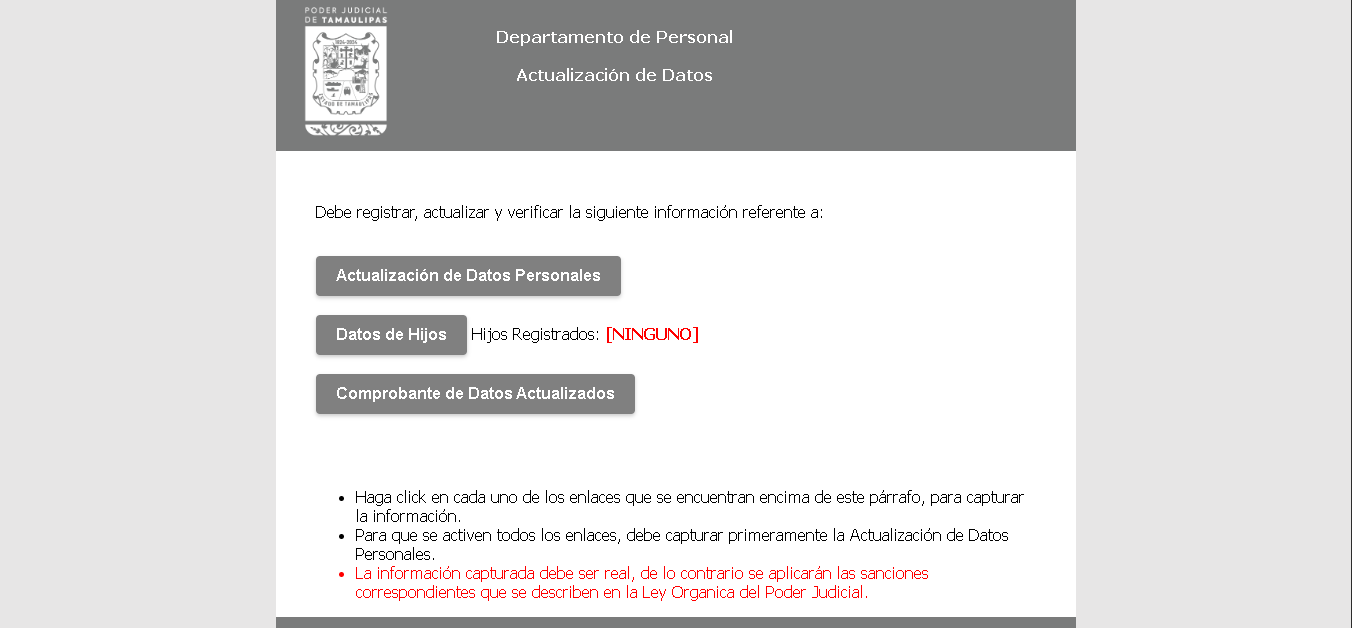
\includegraphics[width=0.9\textwidth]{img/capturasistema.png}
    \caption{Dashboard del Sistema de Actualización de Datos del Personal que se utiliza actualmente en el Poder Judicial de Tamaulipas.}
    \label{fig:sistema_img}
\end{figure}

\subsubsection{Beneficios}
\label{sec:beneficios}

\begin{itemize}
    \item \textbf{Disminución de deuda técnica y mantenibilidad:} Se reemplaza el código monolítico y acoplado del sistema anterior por una estructura limpia basada en la separación de responsabilidades. Esto permitirá que la dirección de informática del Poder Judicial realice modificaciones, correcciones o añada nuevos módulos en el futuro de forma rápida y aislada, sin riesgo de romper otras partes del software.
    \item \textbf{Optimización del rendimiento:} Al eliminar los pesados mecanismos de persistencia en el cliente (ViewState) y los flujos circulares (postbacks) propios de Web Forms, la nueva aplicación web procesará las solicitudes de manera ligera y asíncrona. Esto reducirá drásticamente la carga sobre el servidor del PJETAM y el ancho de banda de la red institucional, garantizando tiempos de respuesta casi inmediatos para los empleados.
    \item \textbf{Fortalecimiento de la seguridad:} La propuesta incluye un esquema de seguridad que remueve los obsoletos proveedores de autenticación del sistema anterior. Se implementará un mecanismo de control de acceso basado en roles (RBAC) y cifrado avanzado de contraseñas para proteger de forma estricta los datos sensibles del personal judicial, asegurando que cada usuario visualice o modifique información exclusivamente de acuerdo con su perfil autorizado.
\end{itemize}

\subsubsection{Recursos Técnicos y de Software}
\label{sec:recursos_tecnicos}

\begin{itemize}
    \item \textbf{Entorno de Desarrollo (IDE):} Microsoft Visual Studio (Edición Enterprise / Community) como plataforma central de codificación.
    \item \textbf{Framework de Desarrollo:} .NET moderno (ASP.NET Core) configurado bajo el patrón MVC.
    \item \textbf{Sistema de Gestión de Base de Datos:} Microsoft SQL Server para la persistencia e integración del repositorio de datos existente. 
    \item \textbf{Herramientas de Mapeo y Migración:} Entity Framework Core integrado mediante la consola de administración de paquetes NuGet.
\end{itemize}

\subsection{Diseño de Interfaz de Usuario}
\label{sec:diseño_interfaz}

\subsubsection{Mockups y Diseños en Figma}
\label{sec:mockups_diseños_figma}
Para empezar con el desarrollo del sistema, primero se definió el diseño de la interfaz del sistema con ayuda de la herramients Figma, ya que esta el útil para crear prototipos interactivos y observar el flujo del sistema antes de empezar a programar.
Para este sistema, no solo se buscó que el diseño fuera más moderno al anterior, sino que se tomó en cuenta el sistema anterior para identificar la información de cada una de la pantallas de los módulos pero también los problemas de usabilidad que surgían.

A partir de esto, se intentó mantener los componentes que ya resultaban familiares para los usuarios, esto para que la transición a este nuevo sistema fuera más sencilla; mientras que para los formularios, se buscó reorganizar la presentación para que los pasos para la navegación fuera menos tediosa.
Durante el diseño también fue importante respetar los lineamientos establecidos en el Manual de Identidad Institucional del Poder Judicial del Estado de Tamaulipas. Se utilizaron los colores oficiales de la institución, la tipografía y el logotipo autorizados, manteniendo así una nueva interfaz moderna pero corporativa y profesional.

\paragraph{Pantalla de Inicio de Sesión} ~\\
\label{sec:inicio_sesion}El diseño para la pantalla de inicio de sesión del anterior sistema tenía una aspecto tradicional y con pocos elementos visuales, por lo que se buscó un diseño más moderno y atractivo, pero sin perder la formalidad.
Se decidió centrar el formulario de autenticación en una interfaz sencilla con los campos de usuario y contraseña. 

De esta manera, se evitan elementos innecesarios que podrían distraer al personal; también se agregó el logotipo institucional y los colores definidos por el Manual de Identidad del Poder Judicial.
El objetivo principal de esta pantalla es reducir la complejidad, y que así el acceso al sistema pueda ser rápido e intuitivo, sin importar si el usuario es nuevo o ya tiene experiencia.

\begin{figure}[H]
    \centering
    \begin{subfigure}[b]{0.45\textwidth}
        
\includegraphics[width=\textwidth]{img/mockup1.png}
        \caption{Mockup del login.}
        \label{fig:mockup_login}
    \end{subfigure}
    \hfill
    \begin{subfigure}[b]{0.45\textwidth}
        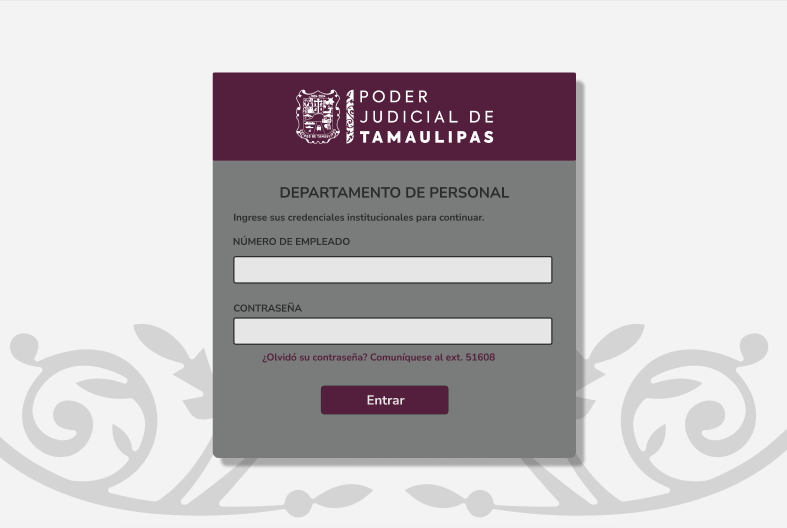
\includegraphics[width=\textwidth]{img/figma1.png}
        \caption{Prototipo de login en Figma.}
        \label{fig:figma_login}
    \end{subfigure}
    \caption{Mockup y prototipo de la pantalla de inicio de sesión del sistema.}
    \label{fig:login_figuras}
\end{figure}

\paragraph{Dashboard} ~\\
\label{sec:dashboard}

\paragraph{Formulario de Datos Personales} ~\\
\label{sec:formulario_datos}

\paragraph{Formulario de Datos de Hijos} ~\\
\label{sec:formulario_hijos}

\paragraph{Comprobante} ~\\
\label{sec:comprobante}



\subsection{Desarrollo del Sistema}
\label{sec:desarrollo_sistema}

\subsubsection{Diagramas de Casos de Uso}
\label{sec:diagramas_casos_uso}

\subsubsection{Diagramas de Bases de Datos}
\label{sec:diagramas_bases_datos}

\subsubsection{Diagramas de Actividades}
\label{sec:diagramas_actividades}

\subsubsection{Diagramas de Secuencia}
\label{sec:diagramas_secuencia}

\clearpage
\input{resultados}

\clearpage
\input{conclusiones}

%\clearpage
%\section*{Bibliografía}
%Agrega las referencias utilizadas.


\clearpage
%\Urlmuskip=0mu plus 1mu\relax
\addcontentsline{toc}{section}{Bibliografía} 
\printbibliography
 
\clearpage
\addcontentsline{toc}{section}{Anexos} 


\thispagestyle{fancy}
%\pagenumbering{roman}
%\setcounter{page}{1}
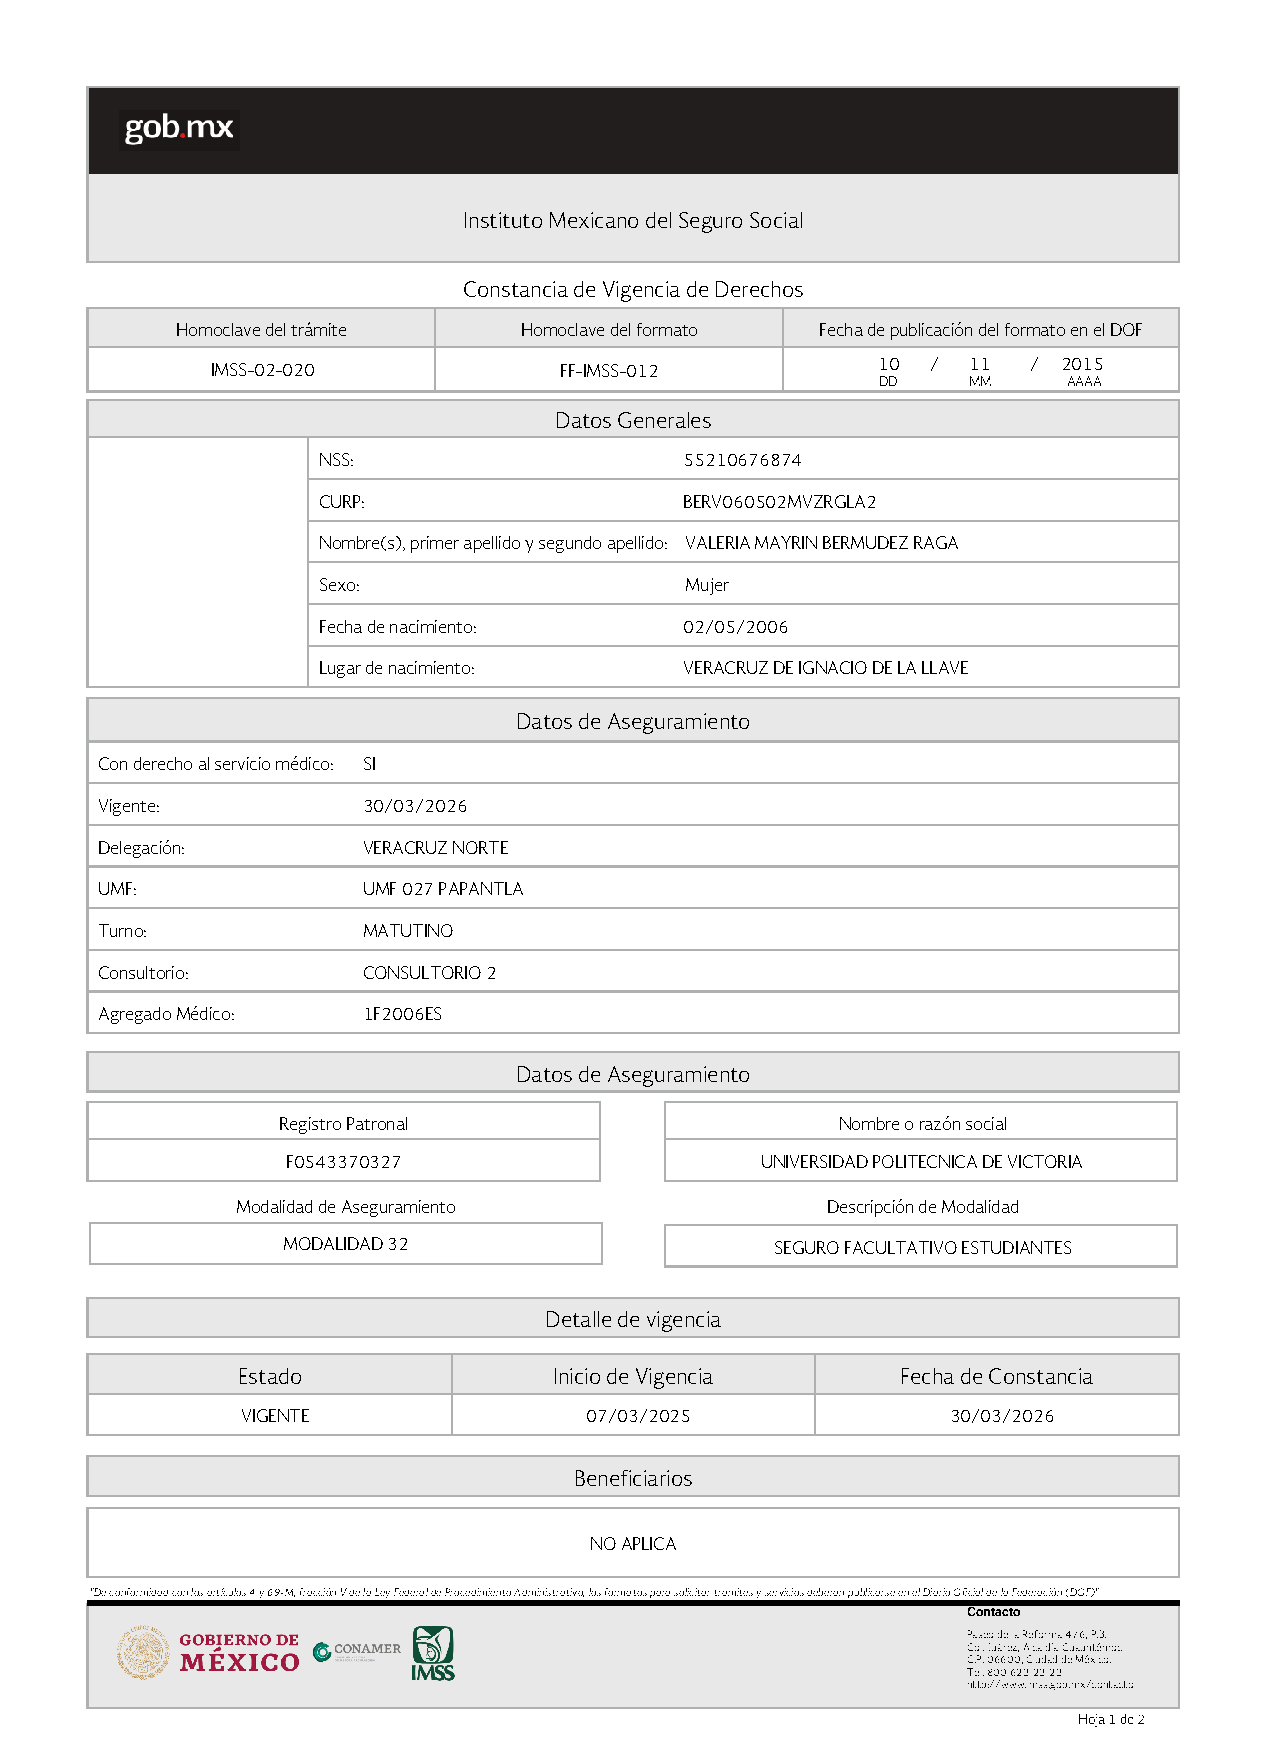
\includepdf[pages={1}]{documentosDigitalizados/SeguroFacultativo.pdf}

% En las siguientes 3 paginas, debe incluir una digitalización de calidad de sus respectivas cartaas, no una fotografia toda cucha tomada con su celular de Coppel
% Pagina 1: Digitalización de la carta de presentación (sustituir por una original en el empastado)
\clearpage
\thispagestyle{fancy}
%\pagenumbering{roman}
%\setcounter{page}{1}

\includepdf[pages={1}]{documentosDigitalizados/CartaPresentacion.pdf}

% Pagina 2: Digitalización de la carta de aceptación (sustituir por una original en el empastado)
\clearpage
\thispagestyle{fancy}
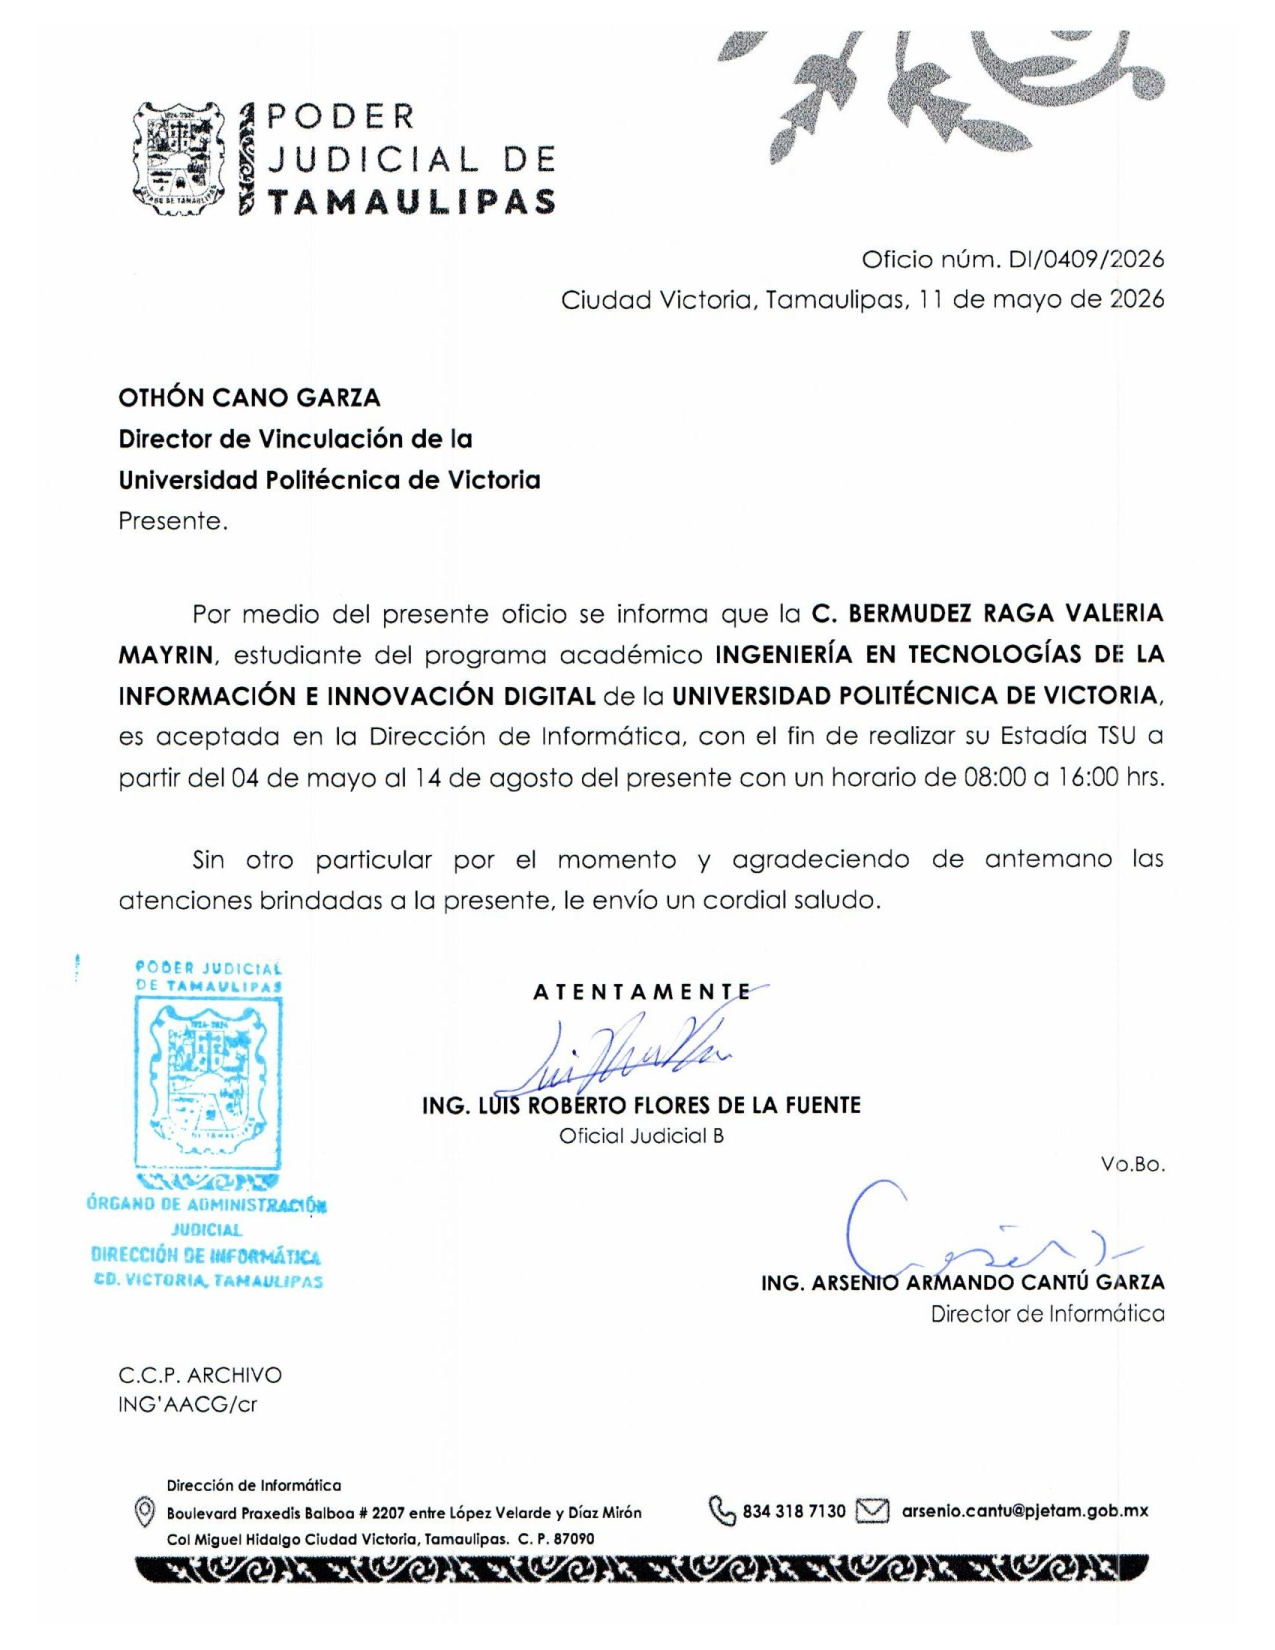
\includepdf[pages={1}]{documentosDigitalizados/CartaAceptacion.pdf}

% Pagina 3: Digitalización de la carta de liberación (sustituir por una original en el empastado)
\clearpage
\thispagestyle{fancy}
\includepdf[pages={1}]{documentosDigitalizados/CartaLiberacion.pdf}

%\chapter*{Rúbrica para la Evaluación del Reporte de Estadía}
\clearpage
%\section*{Rúbrica para la Evaluación del Reporte de Estadía}
\newcommand{\SizeFont}{\footnotesize}

\begin{center}
\large {\textbf{Rúbrica para la Evaluación del Reporte de Estadía}}

\begin{sidewaystable}
\begin{longtable}{|p{0.5cm}|p{13cm}|p{1.5cm}|p{3cm}|}
\hline
%Fecha y lugar en que se emite: \textbf{Ciudad Victoria, Tamaulipas, a \fechaAutorizacionInforme } \\[0.125cm]
\multicolumn{4}{|l|}{Nombre completo del estudiante: \textbf{\NombreAlumno} }\\
\multicolumn{4}{|l|}{Matrícula:  \textbf{\Matricula}}  \\
\multicolumn{4}{|l|}{PERIODO: \ncuatrimestre } \\
\multicolumn{4}{|l|}{Nombre del evaluador: \nasesorinstitucional} \\
\multicolumn{4}{|l|}{ } \\
\multicolumn{4}{|l|}{Firma del Evaluador: \_\_\_\_\_\_\_\_\_\_\_\_\_\_\_\_\_\_\_\_\_\_\_\_  }\\
\multicolumn{4}{|l|}{Calificación Final: \_\_\_ / 100} \\ \hline
Valor & Características a cumplir & Puntos & Observaciones \\ \hline
\SizeFont 6 & \SizeFont Resumen ejecutivo y abstract: Indica qué se realizó, cómo se realizó y qué se obtuvo. (una cuartilla en español e inglés) & & \\ \hline
\SizeFont 6 & \SizeFont Contenido temático: Describe correctamente el contenido del documento & & \\ \hline
\SizeFont 6 & \SizeFont Introducción: El informe cumple con introducir al lector de una manera atractiva el panorama general del trabajo realizado en la unidad económica.  & & \\ \hline
\SizeFont 6 & \SizeFont Descripción de la unidad económica: Se redactan los detalles de los antecedentes del departamento, la empresa, giro, misión, visión, infraestructura, ubicación. & & \\\hline
\SizeFont 6 & \SizeFont Objetivos operativos: Describen las acciones a cumplir mediante actividades establecidas por el asesor empresarial & & \\ \hline
\SizeFont 24 & \SizeFont Metodología: Descripción a detalle de las etapas y procedimientos utilizados en el proyecto & & \\ \hline
\SizeFont 18 & \SizeFont Resultados: Interpreta y analiza los resultados obtenidos durante su estadía. & & \\ \hline
\SizeFont 12 & \SizeFont Conclusiones: Las conclusiones son claras y acordes con el objetivo esperado & & \\ \hline
\SizeFont 6 & \SizeFont Bibliografía y anexos: Cita correctamente las fuentes de información utilizando un estilo de referencia; anexa cartas correspondientes & & \\ \hline
\SizeFont 10 & \SizeFont Responsabilidad: Entregó el reporte en la fecha y hora señalada. Asistió al menos al 80\% de sus días de Estadía & & \\ \hline
\end{longtable}
\end{sidewaystable}

\end{center}

%\chapter*{Rúbrica para Exposición}
\clearpage
\begin{center}
\large {\textbf{Rúbrica para Exposición del Reporte de Estadía}}
\end{center}


\begin{longtable}{|p{3.75cm}|p{3.75cm}|p{3.75cm}|p{3.75cm}|}
\hline
 & \multicolumn{3}{c|}{Nivel de logro} \\ \hline
%A &B  & C & D \\
Criterio &  Bueno ( 10\% ) & Regular (7\% ) & Menor a lo esperado (5\%) \\ \hline
\SizeFont Dominio del tema (10\%) & \SizeFont Utiliza todos los términos y conceptos de manera correcta. & \SizeFont Utiliza la mayoría términos y conceptos de manera correcta & \SizeFont Confunde los términos y conceptos. \\ \hline

\SizeFont  Presentación de material visual (10\%) & \SizeFont Las  diapositivas usadas tienen fondo claro, letras, tablas e imágenes visibles. La presentación contiene los aspectos relevantes de la Estadía
& \SizeFont Las  diapositivas usadas presentan dificultad para su apreciación visual. La presentación contiene los aspectos relevantes de la Estadía & \SizeFont Las  diapositivas usadas presentan dificultad para su apreciación visual. La presentación carece de algunos aspectos relevantes de la Estadía. \\ \hline

\SizeFont   Comunicación y expresión (10\%)  & \SizeFont   Su volumen de voz es comprensible. Su expresión corporal manifiesta seguridad ejecutiva. Su atuendo cumple los estándares de ser formal o semiformal.  Mantiene una línea de respeto en general. &  \SizeFont   Su volumen de voz no es comprensible. Su expresión corporal manifiesta inseguridad. Su atuendo cumple los estándares de ser formal o semiformal.  Mantiene una línea de respeto en general. &
\SizeFont  Su volumen de voz no es comprensible. Su expresión corporal manifiesta inseguridad. Su atuendo no cumple los estándares de ser formal o semiformal.  Realiza alguna falta de respeto. \\ \hline

\SizeFont   Respuestas (10\%) & \SizeFont Las respuestas son consistentes y con parámetros de lógica operativa. & \SizeFont    Las respuestas no son consistentes pero tienen parámetros de lógica operativa. & \SizeFont    Las respuestas son difusas e incoherentes.  \\ \hline


\multicolumn{2}{|c|}{\textbf{Ponderación final de su exposición:}} & \multicolumn{2}{c|}{\_\_\_ /100} \\ \hline
%\multicolumn{2}{|c|}{Día / Mes / Año} &  \multicolumn{2}{c|}{\_\_\_\_ / \_\_\_\_\_\_\_\_ / \_\_\_\_  } \\  \hline
\multicolumn{2}{|c|}{Día / Mes / Año} &  \multicolumn{2}{c|}{\DiaEvaluacionPesentacion / \MesEvaluacionPesentacion / \AnhoEvaluacionPesentacion} \\  \hline
\multicolumn{2}{|c}{ }& \multicolumn{2}{|c|}{ }  \\
\multicolumn{2}{|c}{ }& \multicolumn{2}{|c|}{ }  \\    
\multicolumn{2}{|c}{Comentario adicional} & \multicolumn{2}{|c|}{ } \\  
\multicolumn{2}{|c}{ }& \multicolumn{2}{|c|}{ }  \\  
\multicolumn{2}{|c}{ }& \multicolumn{2}{|c|}{ }  \\  \hline



\end{longtable}

\end{document}








\end{document}
%\section*{Rúbrica para Exposición}
%Completa aquí los criterios de dominio del tema, material visual, comunicación y respuestas.

%\usepackage{longtable}
%\usepackage{array}

\begin{center}
\textbf{RÚBRICA PARA LA EVALUACIÓN DEL REPORTE DE ESTADÍA}
\end{center}

\vspace{0.5cm}

\noindent
\textbf{NOMBRE DEL ESTUDIANTE:} NOMBRES Y APELLIDOS

\noindent
\textbf{PERIODO:} MAYO AGOSTO 2026

\noindent
\textbf{NOMBRE DEL EVALUADOR:} NOMBRES Y APELLIDOS

\noindent
\textbf{FIRMA DEL EVALUADOR:}

\noindent
\textbf{CALIFICACIÓN FINAL:} 60/100

\vspace{0.5cm}

\begin{longtable}{|c|C{7cm}|c|C{4cm}|}
\hline
\textbf{Valor} & \textbf{Características a cumplir} & \textbf{Puntos obtenidos} & \textbf{Observaciones} \\
\hline
6 & Resumen ejecutivo y abstract: Indica qué se realizó, cómo se realizó y qué se obtuvo. (una cuartilla en español e inglés) & & \\
\hline
6 & Contenido temático: Describe correctamente el contenido del documento & & \\
\hline
6 & Introducción: El informe cumple con introducir al lector de una manera atractiva el panorama general del trabajo realizado en la unidad económica. & & \\
\hline
6 & Descripción de la unidad económica: Se redactan los detalles de los antecedentes del departamento, la empresa, giro, misión, visión, infraestructura, ubicación. & & \\
\hline
6 & Objetivos operativos: Describen las acciones a cumplir mediante actividades establecidas por el asesor empresarial & & \\
\hline
24 & Metodología: Descripción a detalle de las etapas y procedimientos utilizados en el proyecto & & \\
\hline
18 & Resultados: Interpreta y analiza los resultados obtenidos durante su estadía. & & \\
\hline
12 & Conclusiones: Las conclusiones son claras y acordes con el objetivo esperado & & \\
\hline
6 & Bibliografía y anexos: Cita correctamente las fuentes de información utilizando un estilo de referencia; anexa cartas correspondientes & & \\
\hline
10 & Responsabilidad: Entregó el reporte en la fecha y hora señalada. Asistió al menos al 80\% de sus días de Estadía & & \\
\hline
\end{longtable}

%\vspace{1cm}

\clearpage
\begin{center}
\textbf{RÚBRICA PARA EXPOSICIÓN DEL REPORTE DE ESTADÍAS}
\end{center}

\begin{center}
\textbf{Técnico Superior Universitario}
\end{center}

\vspace{0.5cm}
\newcommand{\SizeFont}{\small}
\begin{longtable}{|p{3cm}|p{4cm}|p{4cm}|p{4cm}|}
\hline
\textbf{Criterio} & \textbf{Bueno (10\%)} & \textbf{Regular (7\%)} & \textbf{Menor a lo esperado (5\%)} \\
\hline
Dominio del tema & Utiliza todos los términos y conceptos de manera correcta. & Utiliza la mayoría de los términos y conceptos de manera correcta. & Confunde los términos y conceptos. \\
\hline
Presentación de material visual & Las diapositivas tienen fondo claro, con elementos visibles y contienen aspectos relevantes. & Presentan dificultad visual pero incluyen aspectos relevantes. & Presentan dificultad visual y carecen de aspectos relevantes. \\
\hline
Comunicación y expresión & Voz comprensible, seguridad corporal, atuendo formal o semiformal y respeto. & Voz poco comprensible, inseguridad, pero mantiene formalidad. & Voz no comprensible, inseguridad, atuendo inadecuado o falta de respeto. \\
\hline
Respuestas & Respuestas consistentes con lógica operativa. & Respuestas poco consistentes pero con lógica. & Respuestas difusas e incoherentes. \\
\hline
\end{longtable}

\vspace{0.5cm}

\noindent
\textbf{Ponderación final de su exposición:} 40/100

\vspace{0.5cm}

\noindent
\textbf{Datos de la exposición y evaluación}

\noindent
Día / Mes / Año

\noindent
Comentario adicional

\vspace{1cm}

\noindent
Firma \hspace{3cm} Nombre \hspace{3cm} Correo electrónico

\vspace{0.5cm}

\noindent
Profesor asesor institucional

\end{document}
